
\documentclass[10pt,journal,cspaper,compsoc]{IEEEtran}
\hyphenation{op-tical net-works semi-conduc-tor}
\usepackage[pdftex]{graphicx}
\usepackage{url} 
\usepackage{subfig}


\begin{document}

\title{Price Elasticity of the Enterprise Computing Resource Market}

\author
{
Qingye~Jiang,~\IEEEmembership{Senior Member,~IEEE,}
Young Choon~Lee, 
and~Albert~Y.~Zomaya,~\IEEEmembership{Fellow,~IEEE}%
}


\IEEEcompsoctitleabstractindextext{%
\begin{abstract}
Pricing is an important property of a product in that it significantly affects the customer's purchasing behavior. In the enterprise computing resource market, suppliers often compete for market share with price reductions. In many cases, price reductions are the outcome of business intuition rather than rigorous reasoning, and often at the cost of losing revenue and profit. In this paper, we study the supply and demand relationship of the global enterprise computing resource market, using market research data between 2006 and 2013. The market segments we study include the traditional server sales business, server rental business, and public clouds. 
%We find that consumers in different market segments are not equally sensitive to price changes, and we quantitatively measure such sensitivity with the concept of price elasticity of demand. Furthermore, we analyze the success and failure of the major players in the market using the theory of price elasticity of demand.
We find out that the enterprise computing resource market is not a perfect competition market. In the server sales business, IBM, HP and DELL dominate and have the market power over pricing in their respective fine-grained market segment. Consumers in different market segments are not equally sensitive to prices changes. The price elasticity of demand is extremely inelastic for server sales business and server rental business, and is modestly elastic for public clouds. In our case studies with IBM, HP and DELL in the server sales market, price reduction is not an effective way to win market share when the price elasticity of demand is inelastic.
\end{abstract}
\begin{keywords}
enterprise computing resource market, cloud computing, microeconomics, price elasticity of demand
\end{keywords}}

\maketitle
\IEEEdisplaynotcompsoctitleabstractindextext
\IEEEpeerreviewmaketitle

\section{Introduction}
\label{sec:intro}

Pricing strategies are crucial business decisions in the life cycle of a product, especially when there are multiple competitors in the market. In a perfect competition market, there are multiple suppliers offering similar products, while no participant is powerful enough to control the price of the product. To compete for market share, suppliers often use price reduction in promotional campaigns. %However, many of such price reductions are the outcome of business intuition rather than rigorous reasoning, and often at the cost of losing revenue and profit.
To compete for market share, suppliers often use price reduction in promotional campaigns. In order to maintain competitiveness in the market, competitors are forced to lower their prices to match, resulting in a series of pricing wars.  Many of such ``matches''  in price reduction are the outcome of business intuition rather than rigorous reasoning, and often at the cost of losing revenue and profit. It is not uncommon to see enterprises go out of business as the result of pricing wars.

The enterprise computing resource market seems to be a perfect competition market with multiple players. Traditionally, enterprise can buy servers from hardware vendors, or rent servers from hosting service providers. In recent years, Infrastructure-as-a-Service (IaaS) is gradually making its way into the enterprise computing resource market. Amazon Web Services (AWS) are widely recognized as examples of public cloud services. %Over the past years, the market witnessed a trend in developing new applications on AWS, or migrating existing applications to AWS. 
Inspired by the dramatic growth of AWS, there have quickly emerged many followers in the market, including Microsoft Windows Azure and Google Compute Engine. New service providers often employ price reduction as a strategy to win customers from competitors. Existing service providers are forced to carry out further price reductions to maintain competitiveness in the market. In this study, we are particularly interested in the following three questions:

\begin{itemize}
	\item Is the enterprise computing resource market a perfect competition market? 
	\item In the enterprise computing resource market, how sensitive consumers are to price changes?
	\item Is price reduction an effective way to win in the enterprise computing resource market?
\end{itemize}

To answer these questions, we study the supply and demand relationship of the global enterprise computing resource market between 2006 and 2013. We quantitatively measure the consumer's sensitivity to price changes using the concept of price elasticity of demand \cite{marshall}. We analyze the impact of different pricing strategies on the performance of the business, using the server sales business of IBM, HP and DELL as case studies. This research provides new insights into the microeconomics characteristics of the enterprise computing resource market, and can help participants in various market segments design better pricing strategies.

For the server sales business, we collect data from Gartner's quarterly reports on worldwide server shipments between 2006 and 2013. For the server rental business, we use Rackspace as an example of this market segment, and collect data regarding revenue and the number of servers from Rackspace's annual report (Form 10-K) to the United States Securities and Exchange Commission (SEC). For public clouds, we use the estimated number of servers for AWS EC2 derived by a number of cloud computing professionals in the industry as the foundation to carry out our analysis. As the amount of data sources used in this study is overwhelming the limited reference list of this paper, we created a dedicated blog entry \cite{qyjohn} hosted on the author's personal blog site, with links to all the data sources. 

The rest of this paper is organized as follows. Section \ref{sec:background} provides background and related work. In Section \ref{sec:analysis}, we analyze the price elasticity of demand in those three market segments. Section \ref{sec:casestudies} presents case studies on the impact of different pricing strategies, using IBM, HP and DELL as examples. We conclude the paper in Section \ref{sec:conclusions}.

\begin{table*}[t]
\caption{Different Segments in the Enterprise Computing Resource Market}
\label{tbl:resourcemarket}
%\begin{center}
\centering
\begin{tabular}{|p{3cm}|p{4cm}|p{4cm}|p{4cm}|}
\hline
 Market segment& Server Sales Business & Server Rental Business & Public Clouds \\ \hline
Major vendors & IBM, HP, DELL, Fujitsu, Oracle & Rackspace, OVH, SoftLayer & AWS, Google, MS, Rackspace \\ \hline
Acquisition time & weeks & days & minutes  \\ \hline
Expense type & CapEx & OpEx & OpEx \\ \hline
Unit cost  & 2,000--50,000 USD\newline one time payment  & 100--2000 USD\newline monthly charge & 0.02--6.82 USD\newline hourly charge \\ \hline
Ownership & consumer & supplier & supplier \\ \hline
Operations & consumer & supplier & supplier \\ \hline
Life cycle & 3 to 5 years & 1 to 36 months & hourly \\ \hline
Contracts & optional service contract & long term contract with SLA & SLA \\ \hline
Market size (\#servers)& 10M annually or 40M in total & 2M in total & 1M in total \\ \hline
Market share & 93\% & 5\% & 2\% \\ \hline
%Market growth & linear & linear & exponential \\ \hline
\end{tabular}
%\end{center}
\vspace{-10pt}
\end{table*}


\section{Background and Related Work}
\label{sec:background}
In this section, we describe the enterprise computing resource market and discuss related work.

\subsection{The Enterprise Computing Resource Market}
Enterprises have three major options to acquire computing resources. They can either buy new servers from hardware vendors, lease servers from hosting service providers, or use public clouds. The different ways to acquire computing resources represent different segments of the enterprise computing resource market, namely server sales business, server rental business, and public clouds (Table \ref{tbl:resourcemarket}).

\subsubsection{Server Sales Business}
The major suppliers in the server sales business are hardware vendors, including IBM, HP, and DELL. Consumers can order servers directly from the vendors, or through a third-party distributor. The cost to acquire new servers is denoted as capital expense (CapEx), and is usually paid to the supplier in a single payment before or after hardware delivery. The acquisition time usually falls within weeks for low-end servers up to months for high-end servers. When the servers are delivered to the consumer, their ownership is also transferred to the consumer. The life cycle of servers is between three and five years.

\subsubsection{Server Rental Business}
The major suppliers in the server rental business are hosting service providers, including Rackspace, OVH, and SoftLayer. Consumers usually establish a server rental contract directly with the service provider. According to the contract, the consumer pays a recurring monthly fee to maintain access to designated computing resource through network. Such cost is denoted as operations expense (OpEx). The time needed to acquire access to computing resource after signing the contract usually falls within days. The server rental contract does not change the ownership of computing resource, but some service providers choose to give the ownership to the consumer after the successful execution of a long contract (e.g., 3 years). 

\subsubsection{Public Clouds}
Major cloud providers are AWS, Google Compute Engine, Microsoft Windows Azure, and Rackspace. Consumers can directly request for, and gain instant access (within minutes) to, computing resource through web portals or application programming interfaces (API). In a manner similar to public utilities such as gas and electricity, consumers only pay for the amount of computing resource they use for the duration of their usage. The ownership of the physical computing resource always belongs to the service providers. Consumers' responsibility is essentially confined to the pay-as-you-go expense. 

\subsection{Related Work}
There have been several studies on the price elasticity of demand for various computing markets. Due to space limit, we give a selective survey of the literature.

Chow \cite{chow} studies the technological change and the demand for computers with the price and quantity of computers in the United States between 1955 and 1965. Tam et al. \cite{tam} extend Chow's work with annual computer hardware spending data in the United States between 1955 and 1984. Their findings indicate that the price elasticity of demand for computer hardware is inelastic, but the degree of elasticity changes over time. The data sources being used in \cite{chow} are \cite{tam} are extremely old, while technology advancements have dramatically changed the horizon of the computing resource market in general. %These changes not only change the demand for computing resource, but also the relationship between supply and demand. 
On the technology side, expensive mainframes are being replaced by commodity x86\_64 hardware. On the business side, server rental and public clouds are gaining increasing level of popularity among enterprises. Such changes in the demand for computing resource, as well as the relationship between supply and demand, are largely under-explored.

Stavins \cite{stavins} studies the price elasticity of demand for the personal computer market with annual personal computer sales data in the United States between 1976 and 1988. Goolsbee \cite{goolsbee} compares the price sensitivity on computer purchases from online stores versus in retail stores. Both \cite{stavins} and \cite{goolsbee} focus on personal computers instead of enterprise computing resources.

Rogers et al. \cite{451research} use Game Theory to analyze the effect of price reduction on the public cloud market. The authors concluded that there is no Nash equilibrium in this game, resulting in a constant stalemate. Cloud service providers practice price reductions to gain media attention and up-sell value-added services, at the cost of reduced margin from commoditized services such as storage and compute. The problem with this approach is that unless the profit from the value-added services exceeds the lost from down pricing, lowering price always results in reduced profit and can threaten the survival of a business. 

\section{Analysis on Price Elasticity of Demand}
\label{sec:analysis}
In this section, we first introduce the microeconomics concept of price elasticity of demand, describe its application to the enterprise computing resource market. Then, we present our analysis on price elasticity of the three market segments.

\subsection{Price Elasticity of Demand}

Price elasticity of demand is defined by the percentage change in demand over the percentage change in price. More formally,

\begin{equation}
E = \frac{\left ( \frac{dQ}{Q} \right )}{\left ( \frac{dP}{P} \right )} ,
\end{equation}
\\where $E$ represents the price elasticity of demand, $P$ represents the price and $Q$ represents the quantity sold, while $dP$ and $dQ$ represent the percentage changes (in absolute values) in price and demand. When $E$ is greater than 1, the percentage change in demand is greater than the percentage change in price, which is classified as elastic demand. When $E$ is smaller than 1, the percentage change in demand is smaller than the percentage change in price, which is classified as inelastic demand. When $E$ equals to 1, the percentage change in demand equals to the percentage change in price, which is classified as unitary demand. When demand is inelastic, a rise in price leads to a rise in revenue. When demand is elastic, a fall in price leads to a rise in revenue. 

In general, there are two factors contributing to the price elasticity of demand of a product. The first factor is the availability of close substitutes. If a buyer has greater choice among close substitutes in consumption, the price elasticity of demand is greater. The second factor is the proportion of a buyer's budget that is devoted to a product. The larger the proportion of budget, the more responsive is the quantity demanded to price changes, and the price elasticity of demand is greater.

To identify the price elasticity of demand in this study, we carry out linear regression with history price and demand data. With such a technique, we can express the relationship between price and demand as

\begin{equation}
Q = b_0 + b_1 P .
\end{equation}

The slope of a linear curve $b_1$ can also be expressed as

\begin{equation}
b_1 = \frac{dQ}{dP} .
\end{equation}

Therefore

\begin{equation}
\label{eq:elasticity}
E = - b_1  \frac{P}{Q} .
\end{equation}

\begin{figure}[h]
 \subfloat[shipment and revenue]{ 
    \label{fig:shipmentsNrevenue}  
	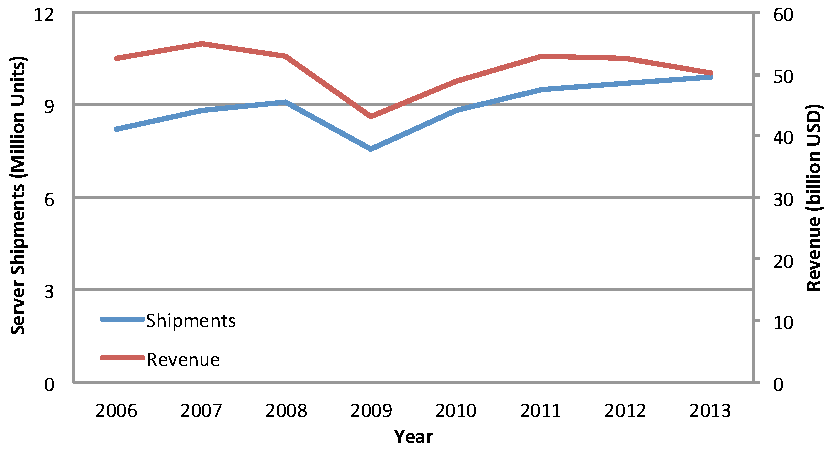
\includegraphics[height=4.5cm]{fig_1_a}}
 \\
 \subfloat[demand curve]{ 
    \label{fig:shipmentsNunitprice}  
	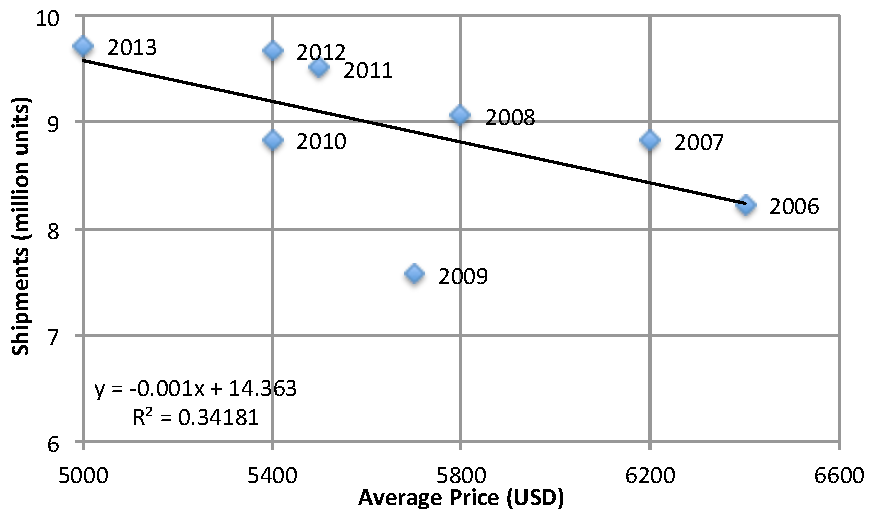
\includegraphics[height=4.5cm]{fig_1_b}}
 \caption{Server Sales Business} 
\end{figure}



\subsection{Price Elasticity of Server Sales Business}
\label{sec:priceServerSales}

We plot annual server shipments and revenue in Figure \ref{fig:shipmentsNrevenue} and show the price elasticity of demand in Figure \ref{fig:shipmentsNunitprice}.
%We plot the number of worldwide server shipments and the revenue generated by the server sales business between 2006 and 2013 in Figure \ref{fig:shipmentsNrevenue} and show the price elasticity of demand in Figure \ref{fig:shipmentsNunitprice}. 
The significant drop in both server shipments and revenue in 2009 was the result of the global economic recession. %, which started in 2008 and ended in 2009. 
Using Equation \ref{eq:elasticity}, the price elasticity of demand for the worldwide server market is calculated as 0.51 in 2013, i.e., extremely inelastic. 

For the majority of enterprise consumers, when they need computing resource the first option that comes to mind is purchasing some server hardware. Other forms of computing resource are not close substitutes for various reasons---renting server hardware from hosting service providers might pose security problems, while public clouds have not been widely adopted. From a budget perspective, server hardware purchases, as fixed-asset investments, are usually decided at the organization level, and are only a small proportion of an organization's annual budget. The lack of close substitutes, and the small proportion of budget, combined contribute to the inelastic demand in server hardware. In other words, organizations invest on server hardware based on their business plans, regardless of price changes in the market. 

A fundamental characteristic of inelastic demand is that the percentage change in demand is less than the percentage change in price. In this case, price reduction might produce more demand, but will also result in revenue lost. In a perfectly monopoly industry, the vendor would always do the opposite, i.e., raising the price and harvesting more revenue. The problem is, the competition in the server hardware market is extremely intensive. Leading server vendors are cutting prices to win market share. Regardless of the steady growth in worldwide server shipments, the overall revenue from server sales seems to be decreasing, as shown in Figure \ref{fig:shipmentsNrevenue}. This results in decreasing margin from server sales, and makes it difficult for server vendors to survive. 


\begin{figure}[t!]
 \subfloat[servers and revenue]{ 
    \label{fig:rackspaceNrevenue}  
	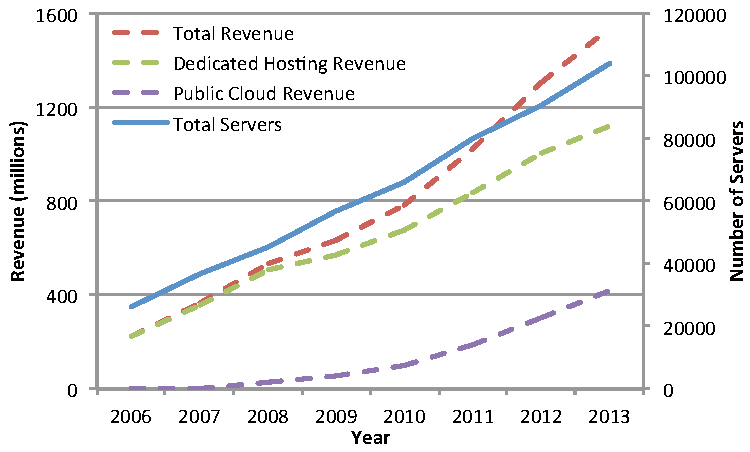
\includegraphics[height=4.5cm]{fig_2_a}}
 \\
 \subfloat[annual server growth and average server price]{ 
    \label{fig:rackspaceNavgrevenue}  
	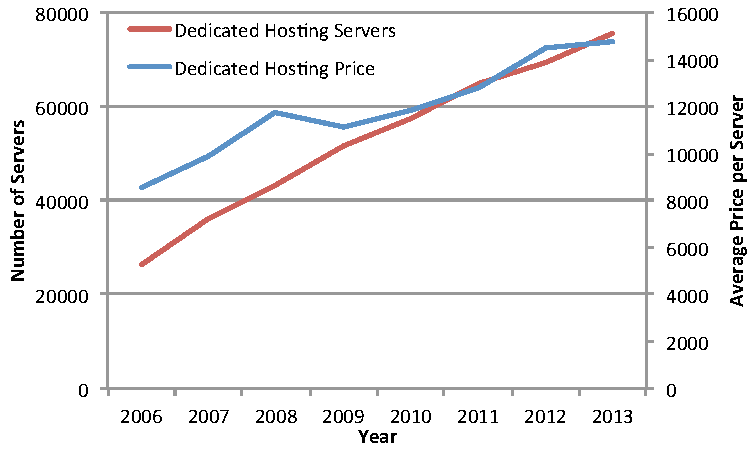
\includegraphics[height=4.5cm]{fig_2_b}}
  \\
 \subfloat[demand curve]{ 
    \label{fig:demandRackspace}  
	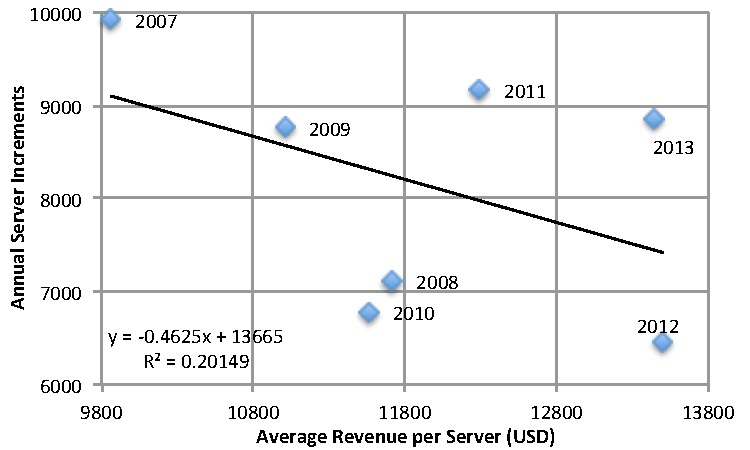
\includegraphics[height=4.5cm]{fig_2_c}}
 \caption{Server Rental Business: Rackspace} 
\end{figure}


\subsection{Price Elasticity of Server Rental Business}

Figure \ref{fig:rackspaceNrevenue} shows Rackspace's number of servers and revenue, as well as the revenue break down for dedicated hosting (server rental business) and public cloud between 2006 and 2013. Figure \ref{fig:rackspaceNavgrevenue} shows the estimated number of servers and the estimated average revenue per server for Rackspace's dedicated hosting business. It should be noted that the number of worldwide server shipments discussed in Section \ref{sec:priceServerSales} represents the newly added computing resource every year. Furthermore, the life cycle of server hardware is usually more than one year, and in most cases falls within the range of three to five years. The number of servers for Rackspace's dedicated hosting business represents the accumulated computing resource over the past years. To facilitate a fair comparison, we calculate the annual server increments for Rackspace's dedicated hosting business, and use that number to compare with the server sales business. Figure \ref{fig:demandRackspace} is a supply and demand plot with the average revenue per server on the horizontal axis and the annual server increments on the vertical axis. The calculated price elasticity of demand for Rackspace's dedicated hosting business is 0.70 in 2013, which is modestly inelastic.

Enterprise consumers choose server rental over buying server hardware for various reasons. For small and medium businesses, the cost and effort to build and maintain a small data center with the appropriate networking capacity is overwhelming. There are many server hosting service providers available, including international and local ones. An enterprise usually needs to go through a comparison and selection process before deciding which one to work with. Once a decision has been made, a long-term contract with the selected service provider will be setup. The length of such contract is usually measured by months or even years, depending on the consumer's business plan. Such a long-term contract effectively eliminates the possibility of migrating to alternative options when there is a price change in the market. Thus, enterprise consumers invest on server rental based on business plans, which are usually not sensitive to price changes. This is why the price elasticity of demand for the server rental business is inelastic. 


\begin{figure}[ht!]
 \subfloat[estimated number of servers for EC2 service]{ 
    \label{fig:shipmentsEC2}  
	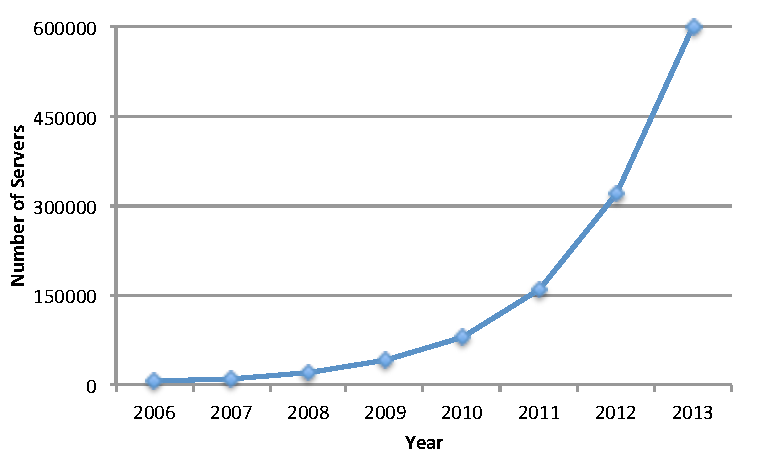
\includegraphics[height=4.5cm]{fig_3_a}}
 \\
 \subfloat[demand curve]{ 
    \label{fig:demandEC2}  
	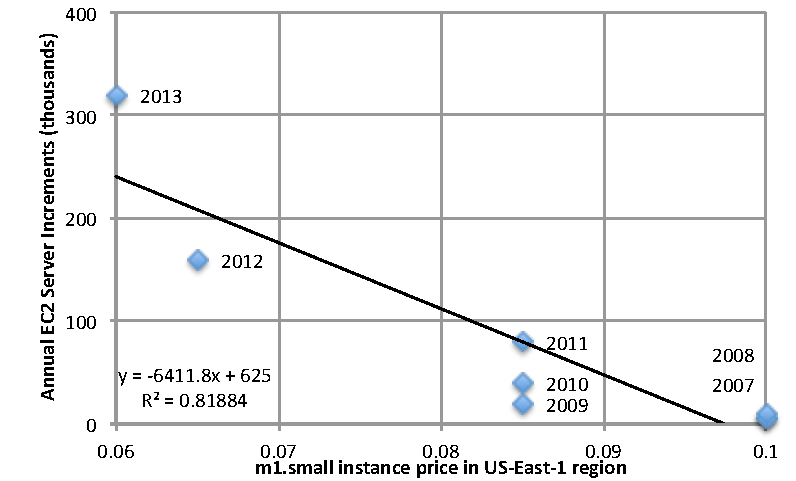
\includegraphics[height=4.5cm]{fig_3_b}}
 \caption{Public Clouds - AWS EC2} 
\end{figure}



\subsection{Price Elasticity of Public Clouds}

For the public cloud business, we use the estimated number of servers for AWS EC2 derived by a number of cloud computing professions in the industry as the foundation to carry out our analysis. AWS is currently the largest public cloud service provider. It is commonly recognized that the size of AWS is far larger than all the competitors combined. Figure \ref{fig:shipmentsEC2} shows the estimated number of servers for AWS EC2 on a global scale. Figure \ref{fig:demandEC2} is a supply and demand plot showing the estimated amount of annual EC2 server increments and the price of m1.small instance in US-East-1 region between 2008 and 2013, with a linear regression trend line. The calculated price elasticity of demand is 1.20 in 2013, which is modestly elastic.

Many consumers consider EC2 as an alternative to traditional server rental services and virtual private server (VPS) services, while ignoring those advanced features such as CloudWatch, AutoScaling, and Elastic Load Balancing. Furthermore, spending on EC2, as an operations expense, is usually decided at the project level, and is usually a big portion of a project's budget. The availability of close substitutes, and the big proportion of budget, combined contribute to the elastic demand for EC2. In other words, enterprise consumers spend on EC2 based on actual business needs rather than business plan, and are sensitive to price changes because of budget limitations.

In general, inelastic demand is closely related to planned buying, while elastic demand is closely related to unplanned buying. With the fixed-asset model, when enterprise consumers need computing resource, the budget for the needed computing resource must first be secured before making an order. Then it takes weeks, if not months, for the needed computing resource to be delivered and deployed. With the utility model, consumers have instant access to computing resource with no capital expense, zero lead time, at affordable prices. In other words, the utility model makes it possible for customers to react to price changes in a timely manner. 

\section{Case Studies}
\label{sec:casestudies}

\begin{figure}[h]
 \subfloat[server shipment and average price]{ 
    \label{fig:shipmentsHPIBMDELL}  
	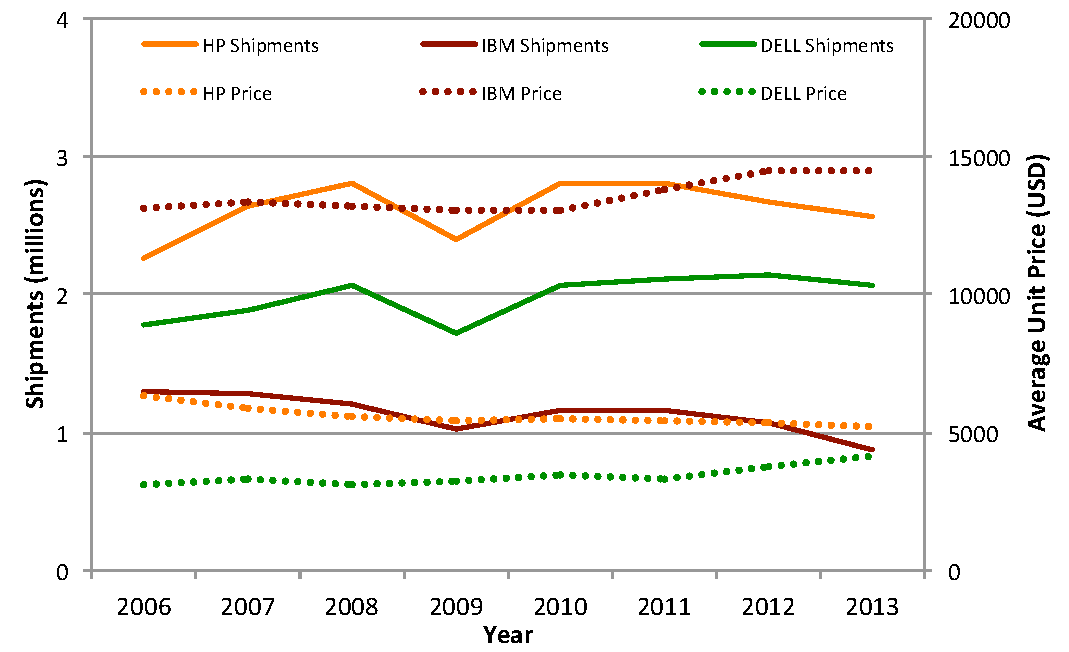
\includegraphics[height=4.5cm]{fig_4_a}}
 \\
 \subfloat[annual revenue]{ 
    \label{fig:revenueHPIBMDELL}  
	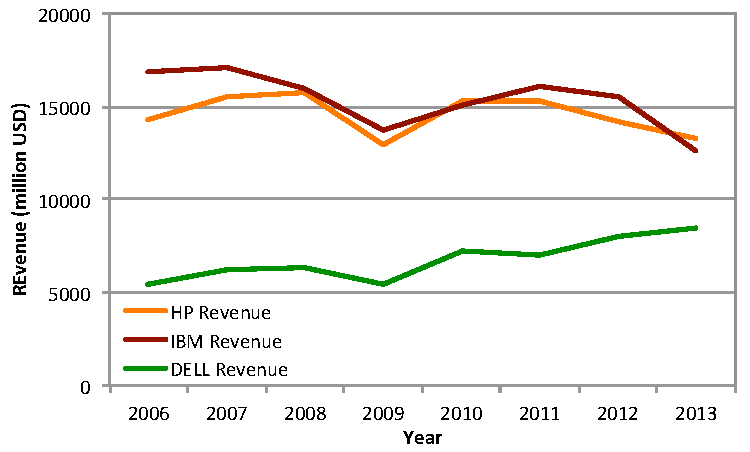
\includegraphics[height=4.5cm]{fig_4_b}}
 \\
 \subfloat[market share]{ 
    \label{fig:shareHPIBMDELL}  
	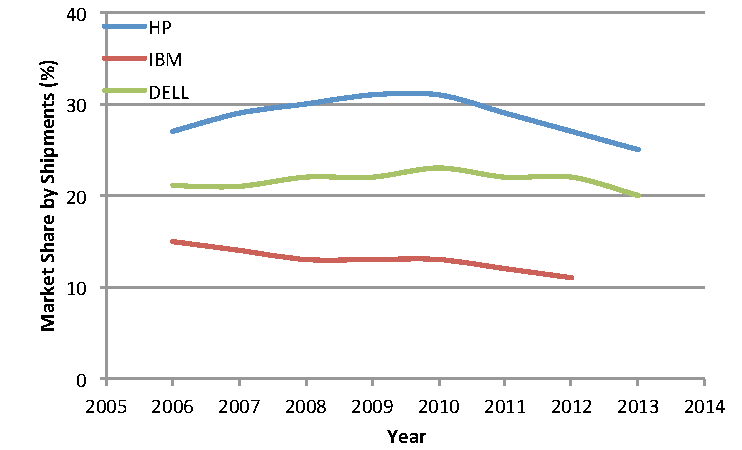
\includegraphics[height=4.5cm]{fig_4_c}}

 \caption{Case Studies: HP, IBM and DELL} 
\end{figure}


In this section, we analyze the impact of different pricing strategies on the performance of the business, using IBM, HP and DELL as case studies; they represent over 75\% of the market share. %There are other vendors in this market segment, including Sun (later acquired by Oracle), Fujitsu, Cisco, etc. Between 2006 and 2013, IBM, HP and DELL combined represent over 75\% of the market share. 

Figure \ref{fig:shipmentsHPIBMDELL} shows the annual server shipments and the average prices for IBM, HP and DELL. The significant gaps in the average prices indicate that these vendors are not competing in the same fine-grained market segment. IBM dominates the high-end server market, HP occupies the mid-range server market, while DELL dominates the low-end server market. 

For IBM, the average price does not change much between 2006 and 2010. The slight decrease in its server shipments is an indicator that the market preference is gradually shifting from high-end servers to mid-range and low-end servers. Between 2010 and 2012, there is an 11\% increase in IBM's average price, with a corresponding 8\% decrease in server shipments. The price elasticity of demand for IBM servers is 0.73, which is modestly inelastic. For HP, there is an 18\% percent decrease in average price between 2006 and 2013, with a corresponding 13\% increase in server shipments. The price elasticity of demand for HP servers is 0.72, which is very similar to IBM. For DELL, there is a 28\% increase in average price, with a corresponding 15\% increase in server shipments. The simultaneous increase in price and shipments indicates that the price elasticity of demand for DELL servers is extremely inelastic - the demand increases regardless of price increases. 

The in-elasticity in demand, plus the significant gaps in the average prices, suggest that enterprise consumers do not perceive IBM, HP and DELL servers as close substitutes for each other. These vendors dominate in their own fine-grained market segment, and have the market power over pricing. IBM responded to the inelastic demand with up-pricing. However, the market preference was shifting from high-end servers to mid-range and low-end servers, resulting in the decrease in revenue. HP responded to the inelastic demand with down-pricing, resulting in increase in shipments but decrease in revenue. DELL responded to the inelastic demand with up-pricing. Coupled with the shift in market preference, DELL achieves a simultaneous increase in server shipments and revenue. The situation for both HP and DELL can be directly derived from Equation (1) - when the demand is elastic, a fall in price leads to a fall in revenue, a rise in price leads to a rise in revenue. Therefore, the HP and DELL cases can be considered as classical examples of how the principle of price elasticity works in microeconomics.

Figure \ref{fig:shareHPIBMDELL} shows the market share for IBM, HP and DELL, as defined by the percentage of server shipments. As shown in this figure, price reduction is not an effective way to win market share.

\section{Conclusions}
\label{sec:conclusions}

In the paper, we study the relationship between price and the amount of computing resources sold on the global enterprise computing resource market, using market research data between 2006 and 2013. We reveal and conclude that:


1. The enterprise computing resource market is not a perfect competition market. In the server sales business, the significant gaps in their average unit prices indicate that the hardware vendors are not competing in the same fine-grained market segment. IBM dominates the high-end server market, HP occupies the mid-range server market, while DELL dominates the low-end server market. These vendors have the market power over pricing in their respective fine-grain market segment.

2. The price elasticity of demand is extremely inelastic for both server sales business and server rental business. Since consumers are not sensitive to price changes, a rise in price leads to a rise in revenue, while a fall in price results in a fall in revenue. The price elasticity of demand is modestly elastic for public clouds. Since consumers are sensitive to price changes, a fall in price results in a rise in revenue.

3. As shown our case studies with IBM, HP and DELL in the server sales market, price reduction is not an effective way to win market share when the price elasticity of demand is inelastic. 

%This paper provides new insights into the microeconomics characteristics of the enterprise computing resource market. It represents the state of the art on the relationship between supply and demand in the enterprise computing resource market. It should be noted that this paper does not take into account factors such as inflation and the natural growth of the enterprise computing resource market. 

\bibliographystyle{ieeetr}  
\bibliography{mybibfile_small}

\begin{IEEEbiographynophoto}{Qingye Jiang}
is pursuing his Master of Phisolophy degree in the School of Information Technologies at The University of Sydney. He is a senior member of IEEE.
\end{IEEEbiographynophoto}

\begin{IEEEbiographynophoto}{Young Choon Lee}
is a Lecturer in the Department of Computing at The University of Sydney.
\end{IEEEbiographynophoto}

\begin{IEEEbiographynophoto}{Albert Y. Zomaya}
is currently the chair professor of high performance computing and networking in the School of Information Technologies, The University of Sydney. He is the author/coauthor of seven books, more than 400 papers, and the editor of nine books and 11 conference proceedings. He is a fellow of IEEE, IET, and AAAS.
\end{IEEEbiographynophoto}

\end{document}